\documentclass[../masters.tex]{subfiles}

\begin{document}
\graphicspath{{./imgs/}{../imgs/}} %look for images

\section{Nonlinear Hybrid Models}
In this section we generalise the graphical model (shown in Figure \ref{fig_hybridmod2} for convenience) of the previous section by dropping the assumption that the dynamic models are linear. The variables retain their meaning as before.     
\begin{figure}[H] 
\centering
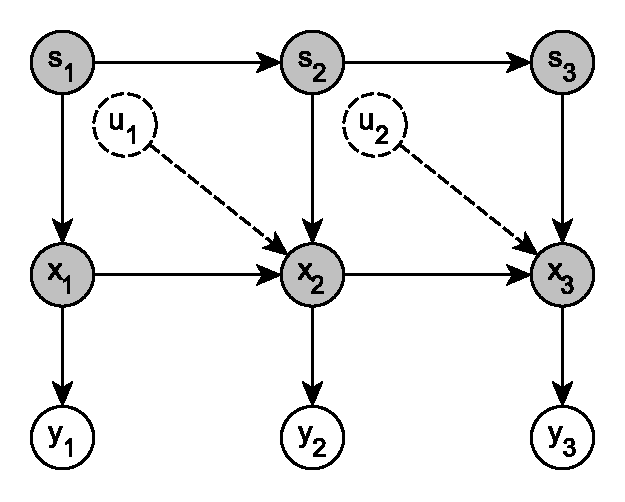
\includegraphics[scale=1.0]{hybrid_model.pdf}
\caption{Graphical model of this section}
\label{fig_hybridmod2}
\end{figure}
Intuitively we are now using the switching variables to decide which nonlinear model better describes the observed system behaviour. At each time point we desire a weighted set of nonlinear models with the weight proportional to the ability of the model to explain the plant behaviour. Such a system could be used to describe significant model changes e.g. catalyst degradation in our CSTR or a reactor which breaks suddenly etc... 

We model this system as follows. Let $s_t=1,2,..., N$ denote a discrete, time homogeneous $N$ state first order Markov chain with transition matrix $P$ as discussed in the previous section. Let each state $s_t=i$ be associated with a model set $\left(f_i, g_i, Q_i, R_i \right)$ used to evaluate the dynamical model shown in (\ref{eq_smodel}).
\begin{equation}
\begin{aligned}
x_{t+1} &= f_i(x_t, u_t, w_{t+1}) \text{ with } w_{t+1} \backsim \mathcal{N}(0, Q_i)\\
y_{t+1} &= g_i(x_{t+1}, v_{t+1}) \text{ with } v_{t+1} \backsim \mathcal{N}(0,R_i)
\end{aligned}
\label{eq_smodel}
\end{equation}
In this dissertation we assume that the the noise distributions are Gaussian but there is no fundamental reason why they cannot be arbitrary. To fully specify the system we again require the prior distributions $p(s_1)$ and $p(x_1|s_1)$ as well as the stochastic matrix $P$. In this section we manually specify the matrix $P$. 

\subsection{Exact Inference}
By extending the model to incorporate nonlinear models it becomes even more difficult to perform inference. It is clear that for the type of systems we consider here no exact inference algorithm which is computationally feasible exists. We again turn to approximate inference algorithms.

Note that we cannot apply Rao-Blackwellisation (i.e. analytically evaluate the stochastic dynamical system) as before because the dynamic models are no longer linear. We use the adaptive Sequential Importance Resampling (i.e. the bootstrap) Particle Filter algorithm as discussed in the Nonlinear Models section.

\subsection{Approximate Inference}
We cannot analytically evaluate any part of the desired posterior distribution $p(s_{1:t}, x_{1:t}|y_{1:t})$ in a computationally feasible manner, so we must apply the adaptive Sequential Importance Resampling algorithm to the entire state space of Figure \ref{fig_hybridmod2}. The algorithm follows straightforwardly from our previous discussion \cite{murphy1}. We merely state the incremental weight function and proposal distribution we sample from in (\ref{eq_nonpf}). 
\begin{equation}
\begin{aligned}
&q_t(s_t,x_t|s_{1:t-1},x_{1:t-1,}y_{1:t}) = p(s_t|s_{t-1})p(x_t|s_t,x_{t-1}) \\
&\alpha_t(s_{1:t},x_{1:t}) = p(y_t|x_t,s_t)
\end{aligned}
\label{eq_nonpf}
\end{equation}  
Applying the algorithm is a straightforward extension of the bootstrap filter shown in the Nonlinear Models section given the weighting function and proposal distribution as shown below.

\textbf{Switching Particle Filter Algorithm}\\
For $t=1$:
\begin{enumerate}
\item
Sample $S^i_1 \backsim p(s_1)$ and $X^i_1 \backsim p(x_1|s_1)$.
\item
Compute the weights $w_1(S_1^i, X_1^i) = p(Y^*_1|S_1^i, X_1^i)$ where $Y^*_1$ is the observation. Normalise $W^i_1 \propto w_1(S_1^i, X_1^i)$. 
\item
If the number of effective particles is below some threshold apply resampling with roughening $(W^i_1, S^i_1, X^i_1)$ to obtain $N$ equally weighted particles $(\frac{1}{N}, \bar{S}^i_1, \bar{X}^i_1)$ and set $(\bar{W}^i_1, \bar{S}^i_1,\bar{X}^i_1) \leftarrow (\frac{1}{N}, \bar{S}^i_1, \bar{X}^i_1)$ otherwise set $(\bar{W}^i_1,\bar{S}^i_1, \bar{X}^i_1) \leftarrow ({W}^i_1, S_1^i, {X}^i_1)$
\end{enumerate}
For $t \geq 2$:
\begin{enumerate}
\item
Sample $S^i_t \backsim p(S_t^i|\bar{S}^i_{t-1})$ and $X^i_t \backsim p(X^i_t|S^i_t, \bar{X}^i_{t-1})$.
\item
Compute the weights $\alpha_t(S_t^i, X_t^i) = p(Y^*_t|S_t^i, X_t^i)$ where $Y^*_t$ is the observation. Normalise $W^i_t \propto W^i_{t-1}\alpha_t(S_t^i, X_t^i)$.
\item
If the number of effective particles is below some threshold apply resampling with roughening $(W^i_1, S^i_t, X^i_t)$ to obtain $N$ equally weighted particles $(\frac{1}{N}, \bar{S}^i_t, \bar{X}^i_t)$ and set $(\bar{W}^i_t, \bar{S}^i_t,\bar{X}^i_t) \leftarrow (\frac{1}{N}, \bar{S}^i_t, \bar{X}^i_t)$ otherwise set $(\bar{W}^i_t,\bar{S}^i_t, \bar{X}^i_t) \leftarrow ({W}^i_t, S_t^i, {X}^i_t)$
\end{enumerate} 

\subsection{Particle Prediction}
The prediction of the hybrid nonlinear states follows in an analogous manner to the prediction of the Nonlinear Models seen in the previous sections. We do not supply an algorithm because it is a straightforward simplification of the Switching Particle Filter algorithm seen above (effectively there is no weight update step).  

\subsection{Filtering the CSTR}
In this section we illustrate the use of the Switching Particle Filter using nonlinear dynamical models. We assume a scenario where the rate constant of the CSTR decreases by an order of magnitude. This could be caused by catalyst degradation due to some environmental factor. It is our aim to infer when this happens and to be able to track the states accurately despite the significant model change. 

We use 500 particles during all runs and use the stochastic matrix $P=\begin{pmatrix}
0.9 & 0.1 \\ 0.1 & 0.9
\end{pmatrix}.$ The form of the matrix is motivated by physical considerations: once the catalyst denatures it is unlikely to fix itself. Thus, the matrix reflects a situation where a state is not likely to jump to another state. In all the simulations the catalyst denatures at 40 minutes into the run.

First we investigate a situation where only the temperature is measured. Second we include a concentration measurement and third we investigate the benefit of adding the second state measurement. Consider Figures \ref{fig_spf_m1_s} and \ref{fig_spf_m1_t} which show the Switching Particle Filter at work using only one measurement. 

Based on Figure \ref{fig_spf_m1_s} it is evident that the first model (with the catalyst at full effectiveness) is the dominant model until about 40 minutes into the simulation. There is an abrupt change as the filter realises that first model no longer describes the system well and it switches to the second model. Up to about 120 minutes into the simulation the second model dominates. We then see a gradual decrease in the prominence of the second model. 
\begin{figure}[H] 
\centering
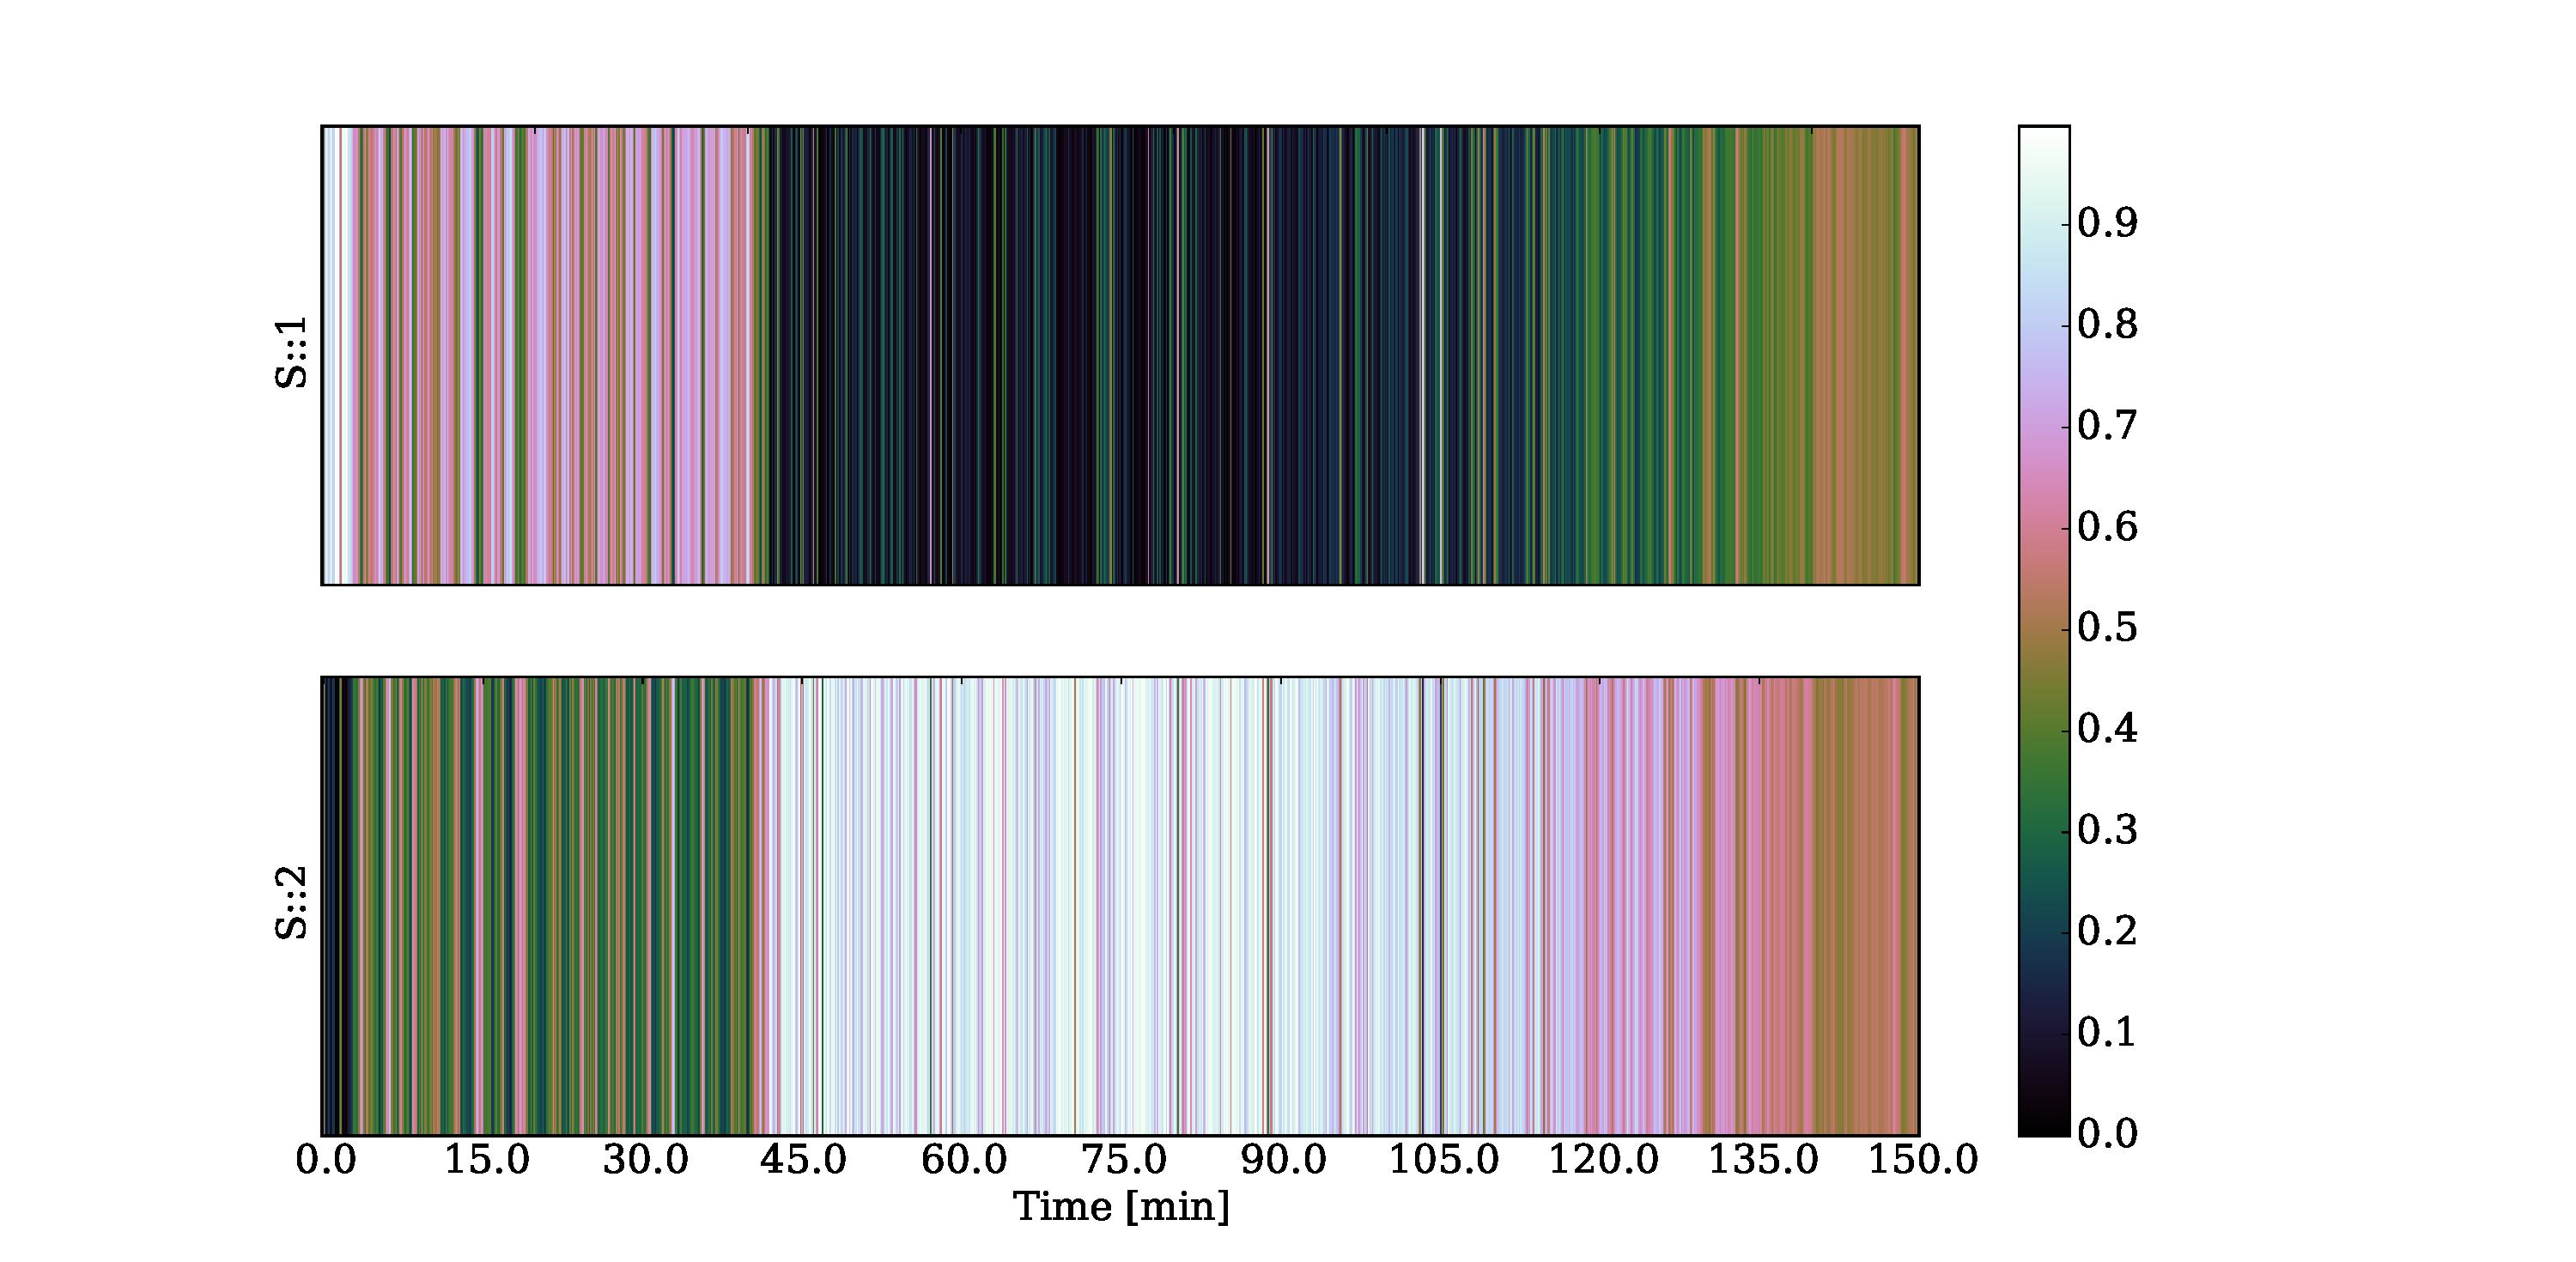
\includegraphics[scale=0.3]{spf_m1_s.pdf}
\caption{Weight of each switching index as time progresses. The catalyst denatures at 40 min.}
\label{fig_spf_m1_s}
\end{figure}
This is exactly the type of behaviour we expected except, perhaps, the gradual decrease near the end of the simulation. The reason why this happens is because at high concentrations and low temperatures both models drive the system to the same steady state concentration. Therefore we see that both models explain the data.

In Figure \ref{fig_spf_m1_t} we see the transient response of the system. The green dashed line indicates the trajectory of the system if the catalyst did not denature.  
\begin{figure}[H] 
\centering
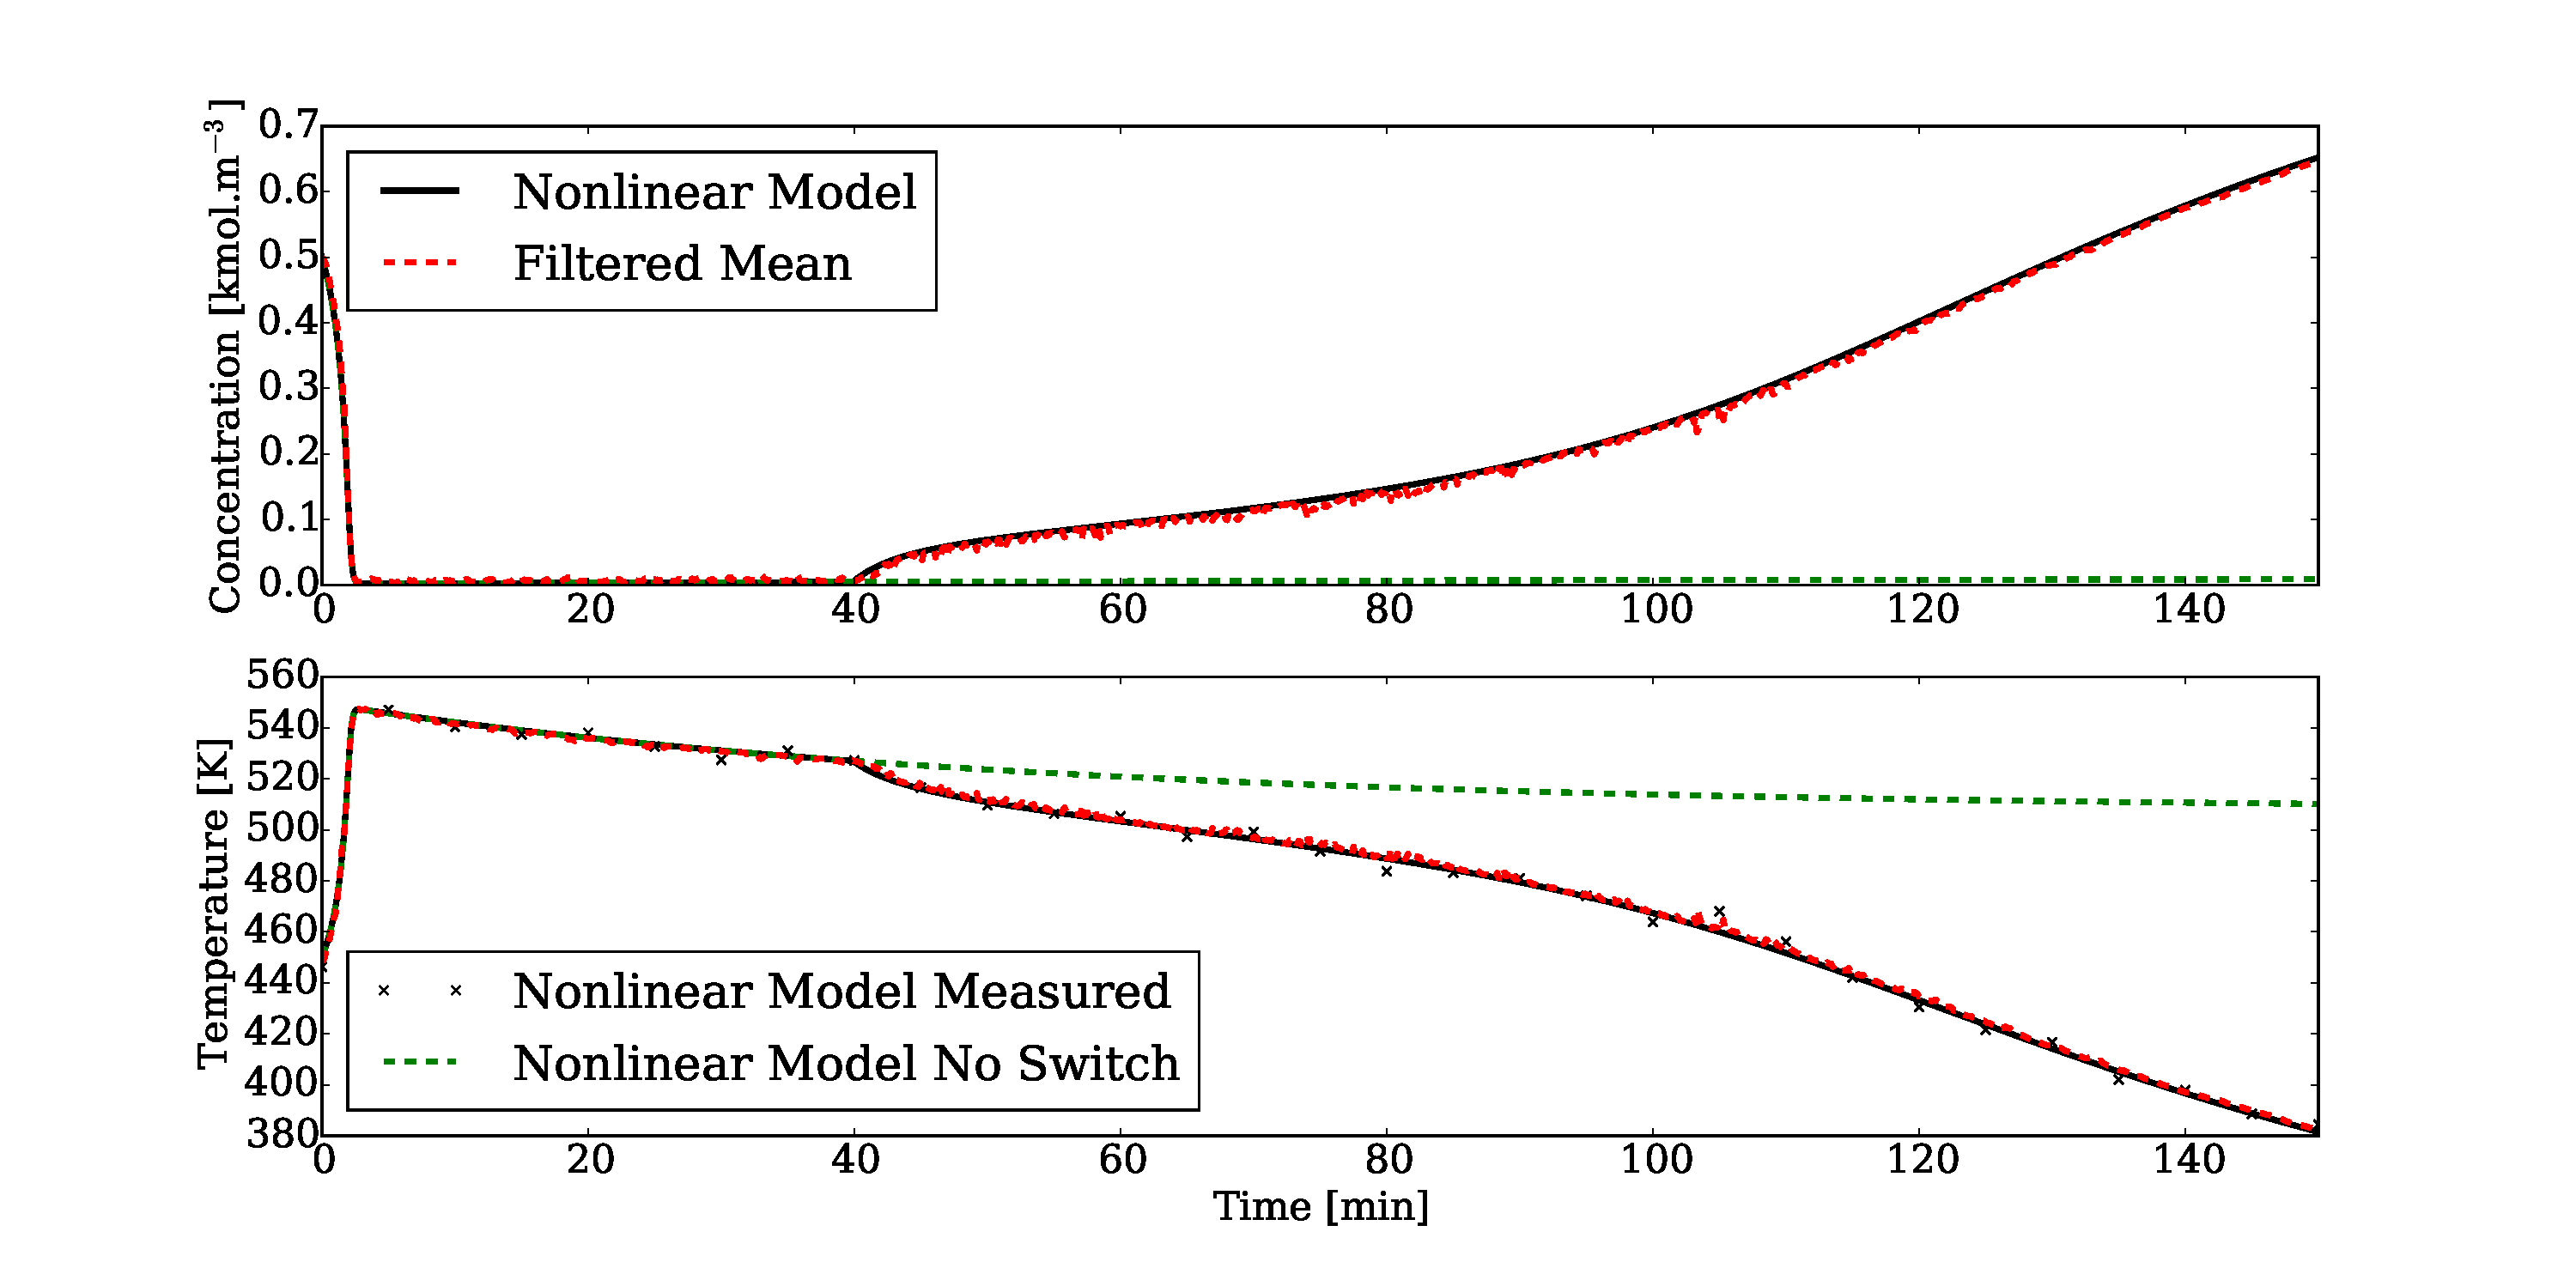
\includegraphics[scale=0.3]{spf_m1_t.pdf}
\caption{Time series evolution of the states with initial condition ($0.5, 450$). The catalyst denatures at 40 min.}
\label{fig_spf_m1_t}
\end{figure}
We see that the Switching Particle Filter accuracy tracks both temperature and concentration. The high accuracy of the model causes the concentration, although unmeasured, to be inferred accurately. We expect that if the models were not as accurate the inference would suffer.

Next we consider Figures \ref{fig_spf_m2_s} and \ref{fig_spf_m2_t} which shows the filter at work using both temperature and concentration state measurements. In Figure \ref{fig_spf_m2_s} we see much the same behaviour as Figure \ref{fig_spf_m1_s}.
\begin{figure}[H] 
\centering
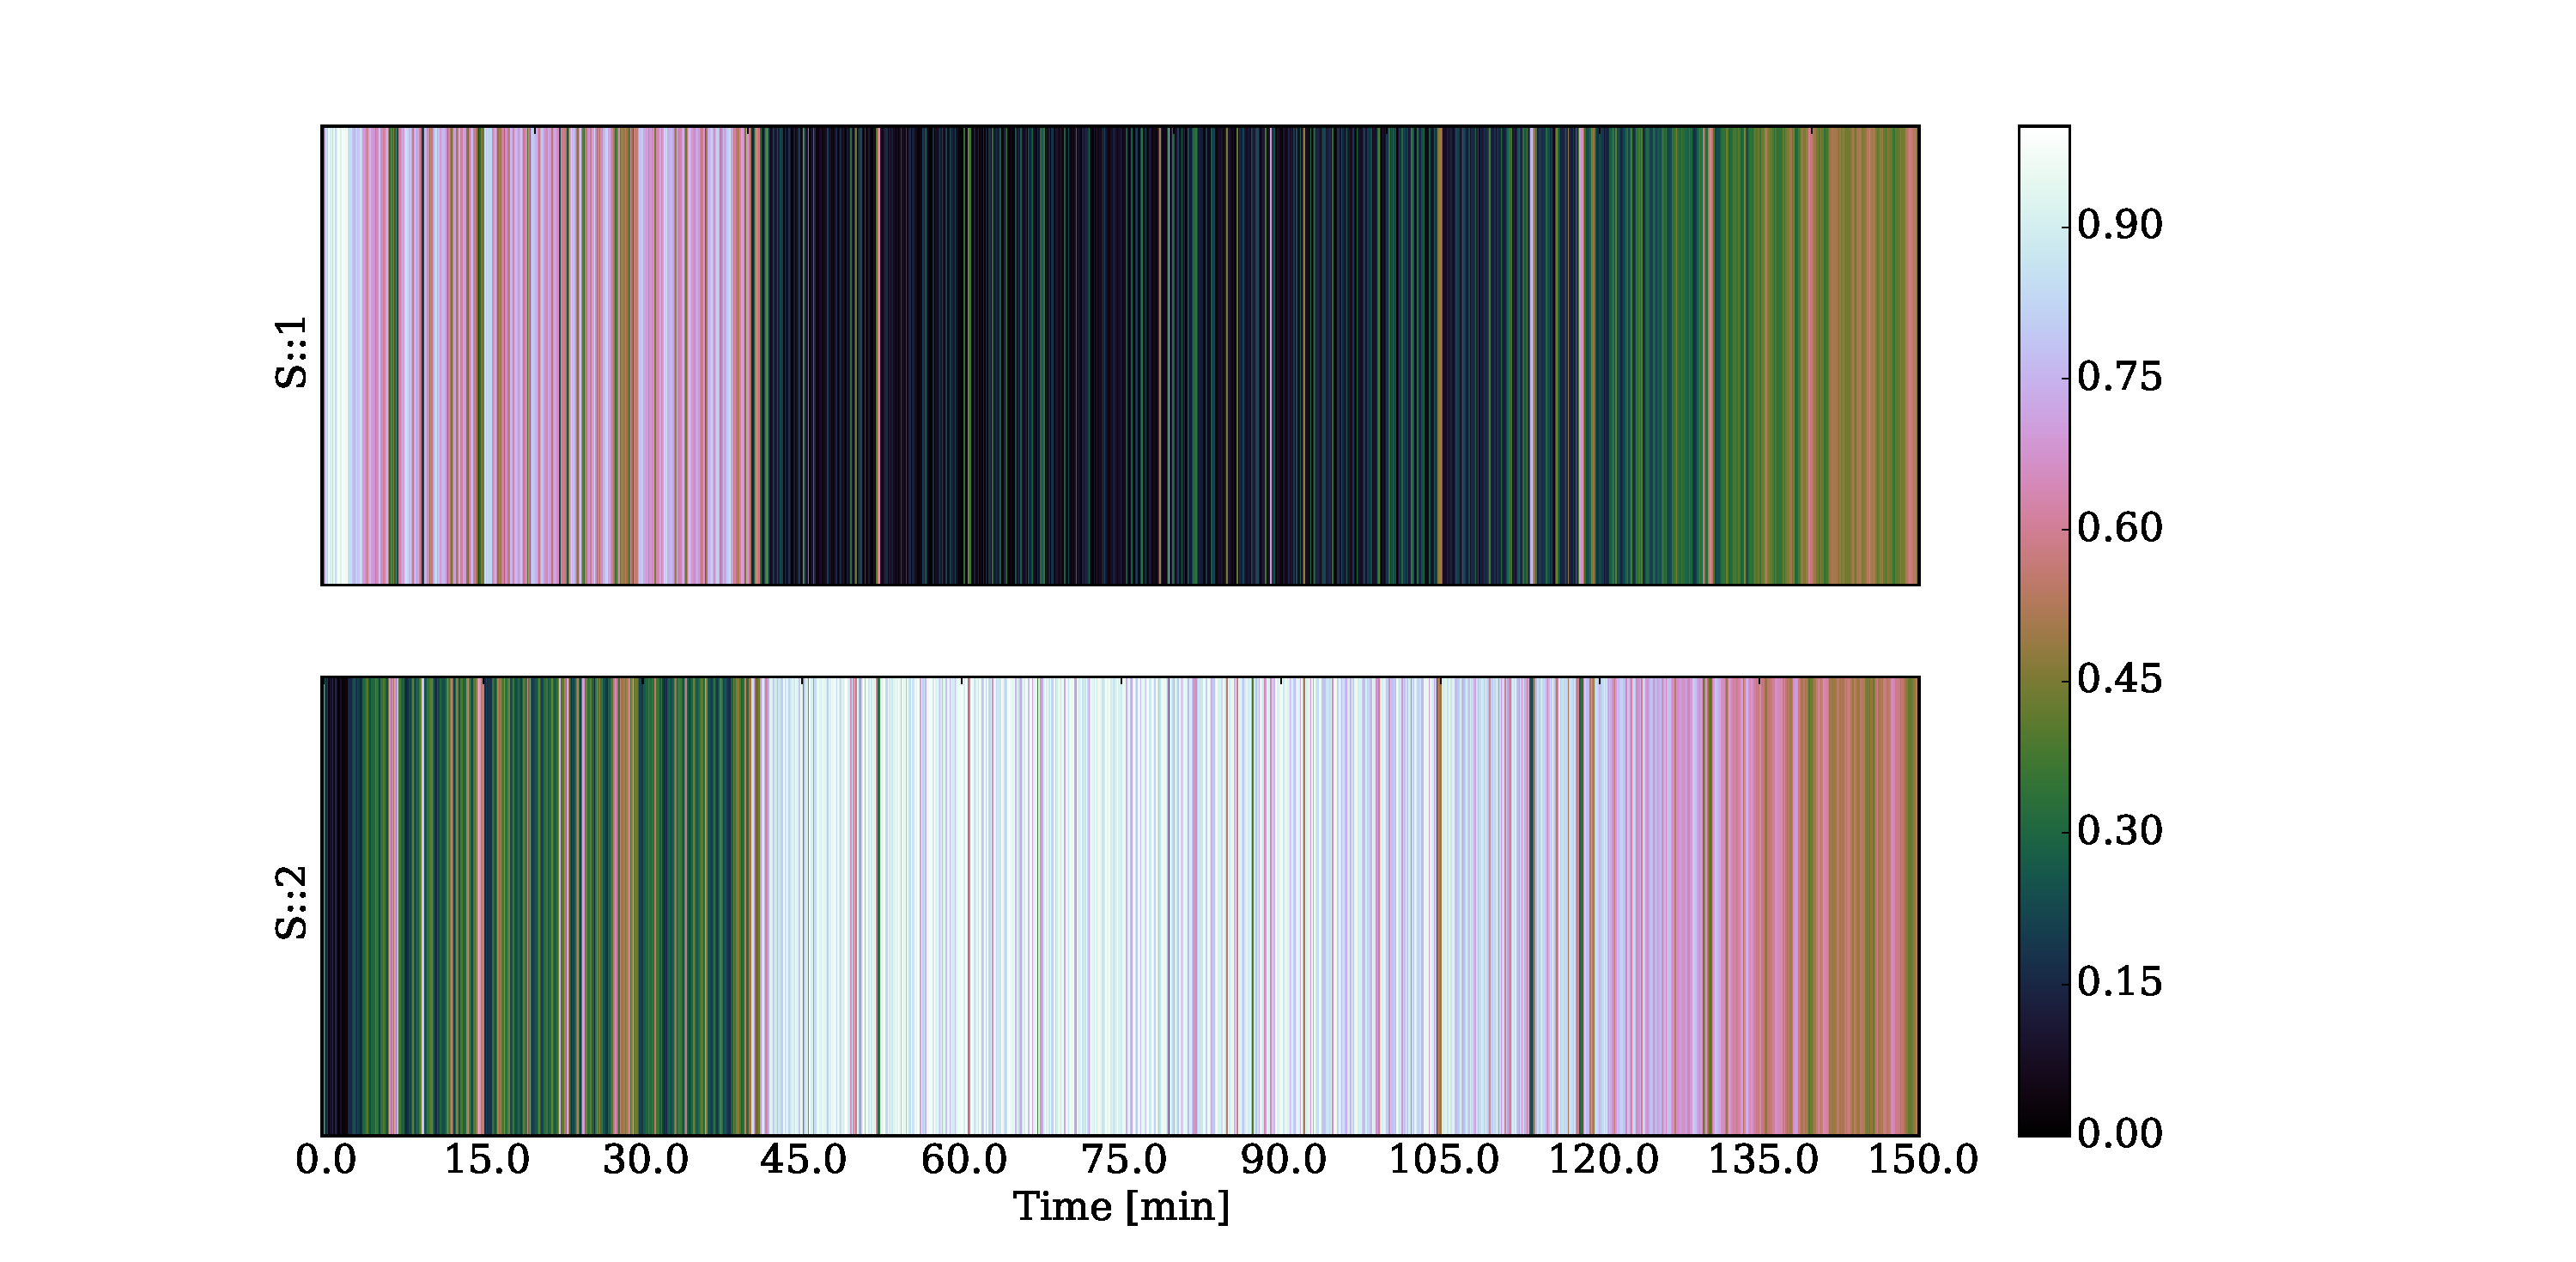
\includegraphics[scale=0.3]{spf_m2_s.pdf}
\caption{Weight of each switching index as time progresses. The catalyst denatures at 40 min.}
\label{fig_spf_m2_s}
\end{figure}
In Figure \ref{fig_spf_m2_t} we see the transient response of the system. Again the filter is able to accurately track the system states.
\begin{figure}[H] 
\centering
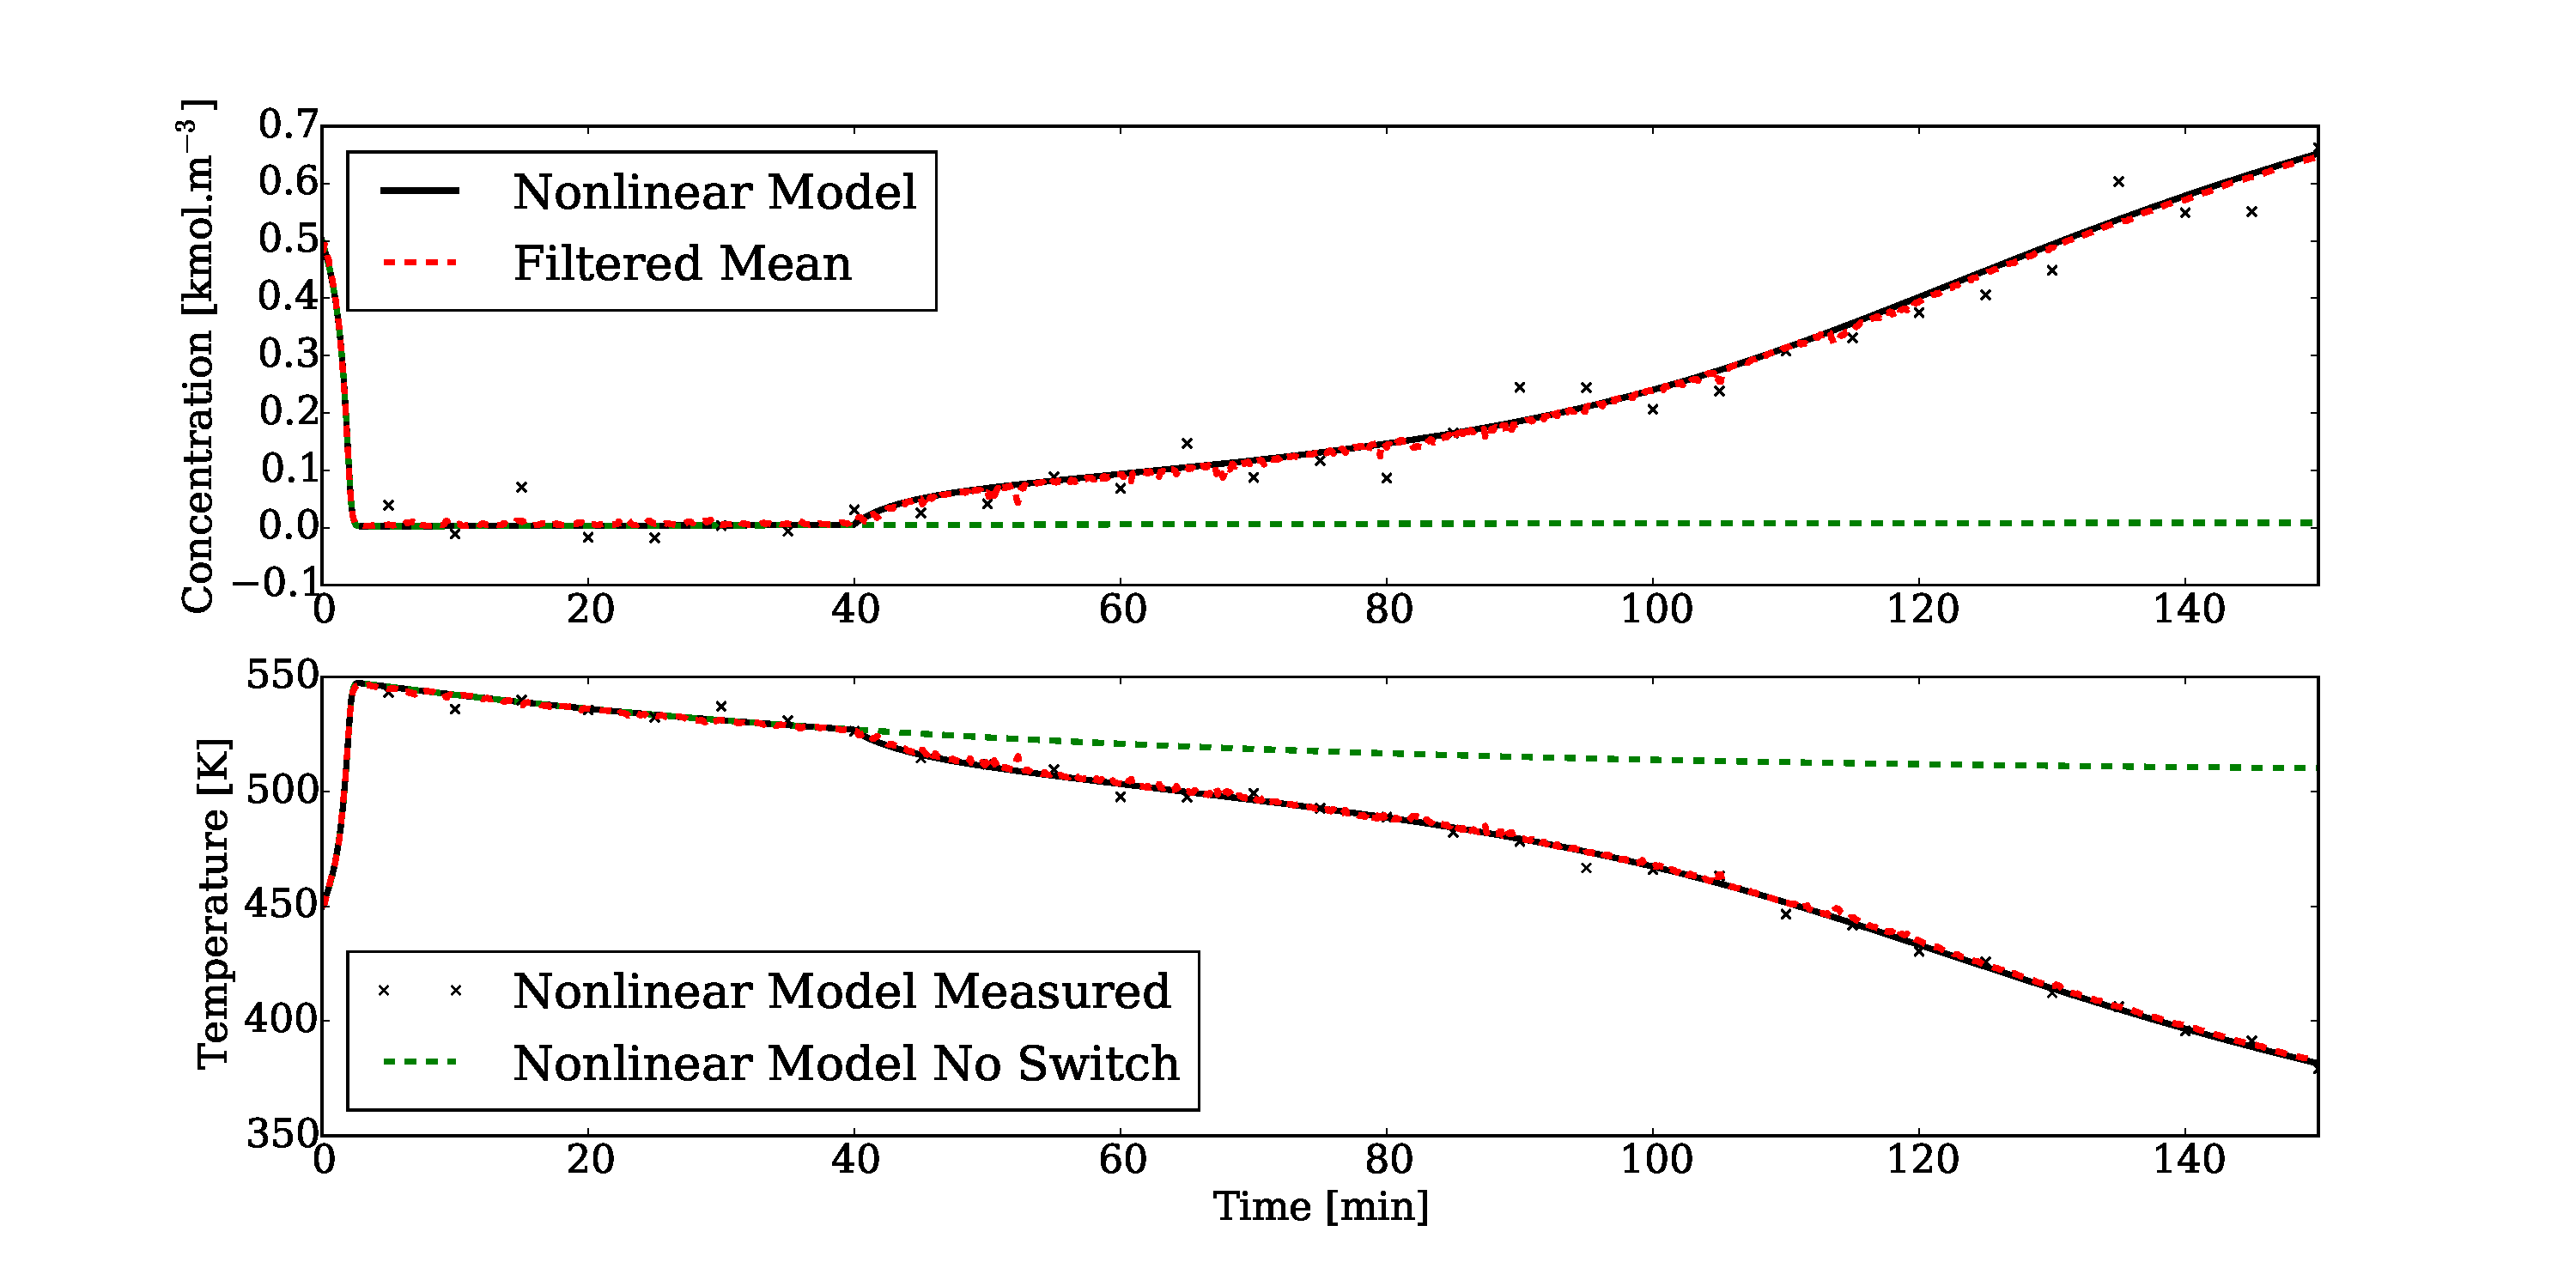
\includegraphics[scale=0.3]{spf_m2_t.pdf}
\caption{Time series evolution of the states with initial condition ($0.5, 450$). The catalyst denatures at 40 min.}
\label{fig_spf_m2_t}
\end{figure}
Generally speaking the second measurement will increase the filter accuracy if the models are not accurate. It is not clear if there is a tangible benefit to using the second measurement in this case. To this end we introduce Figure \ref{fig_spf_m1_m2} which compares the posterior state estimates using one and two measurements. 
\begin{figure}[H] 
\centering
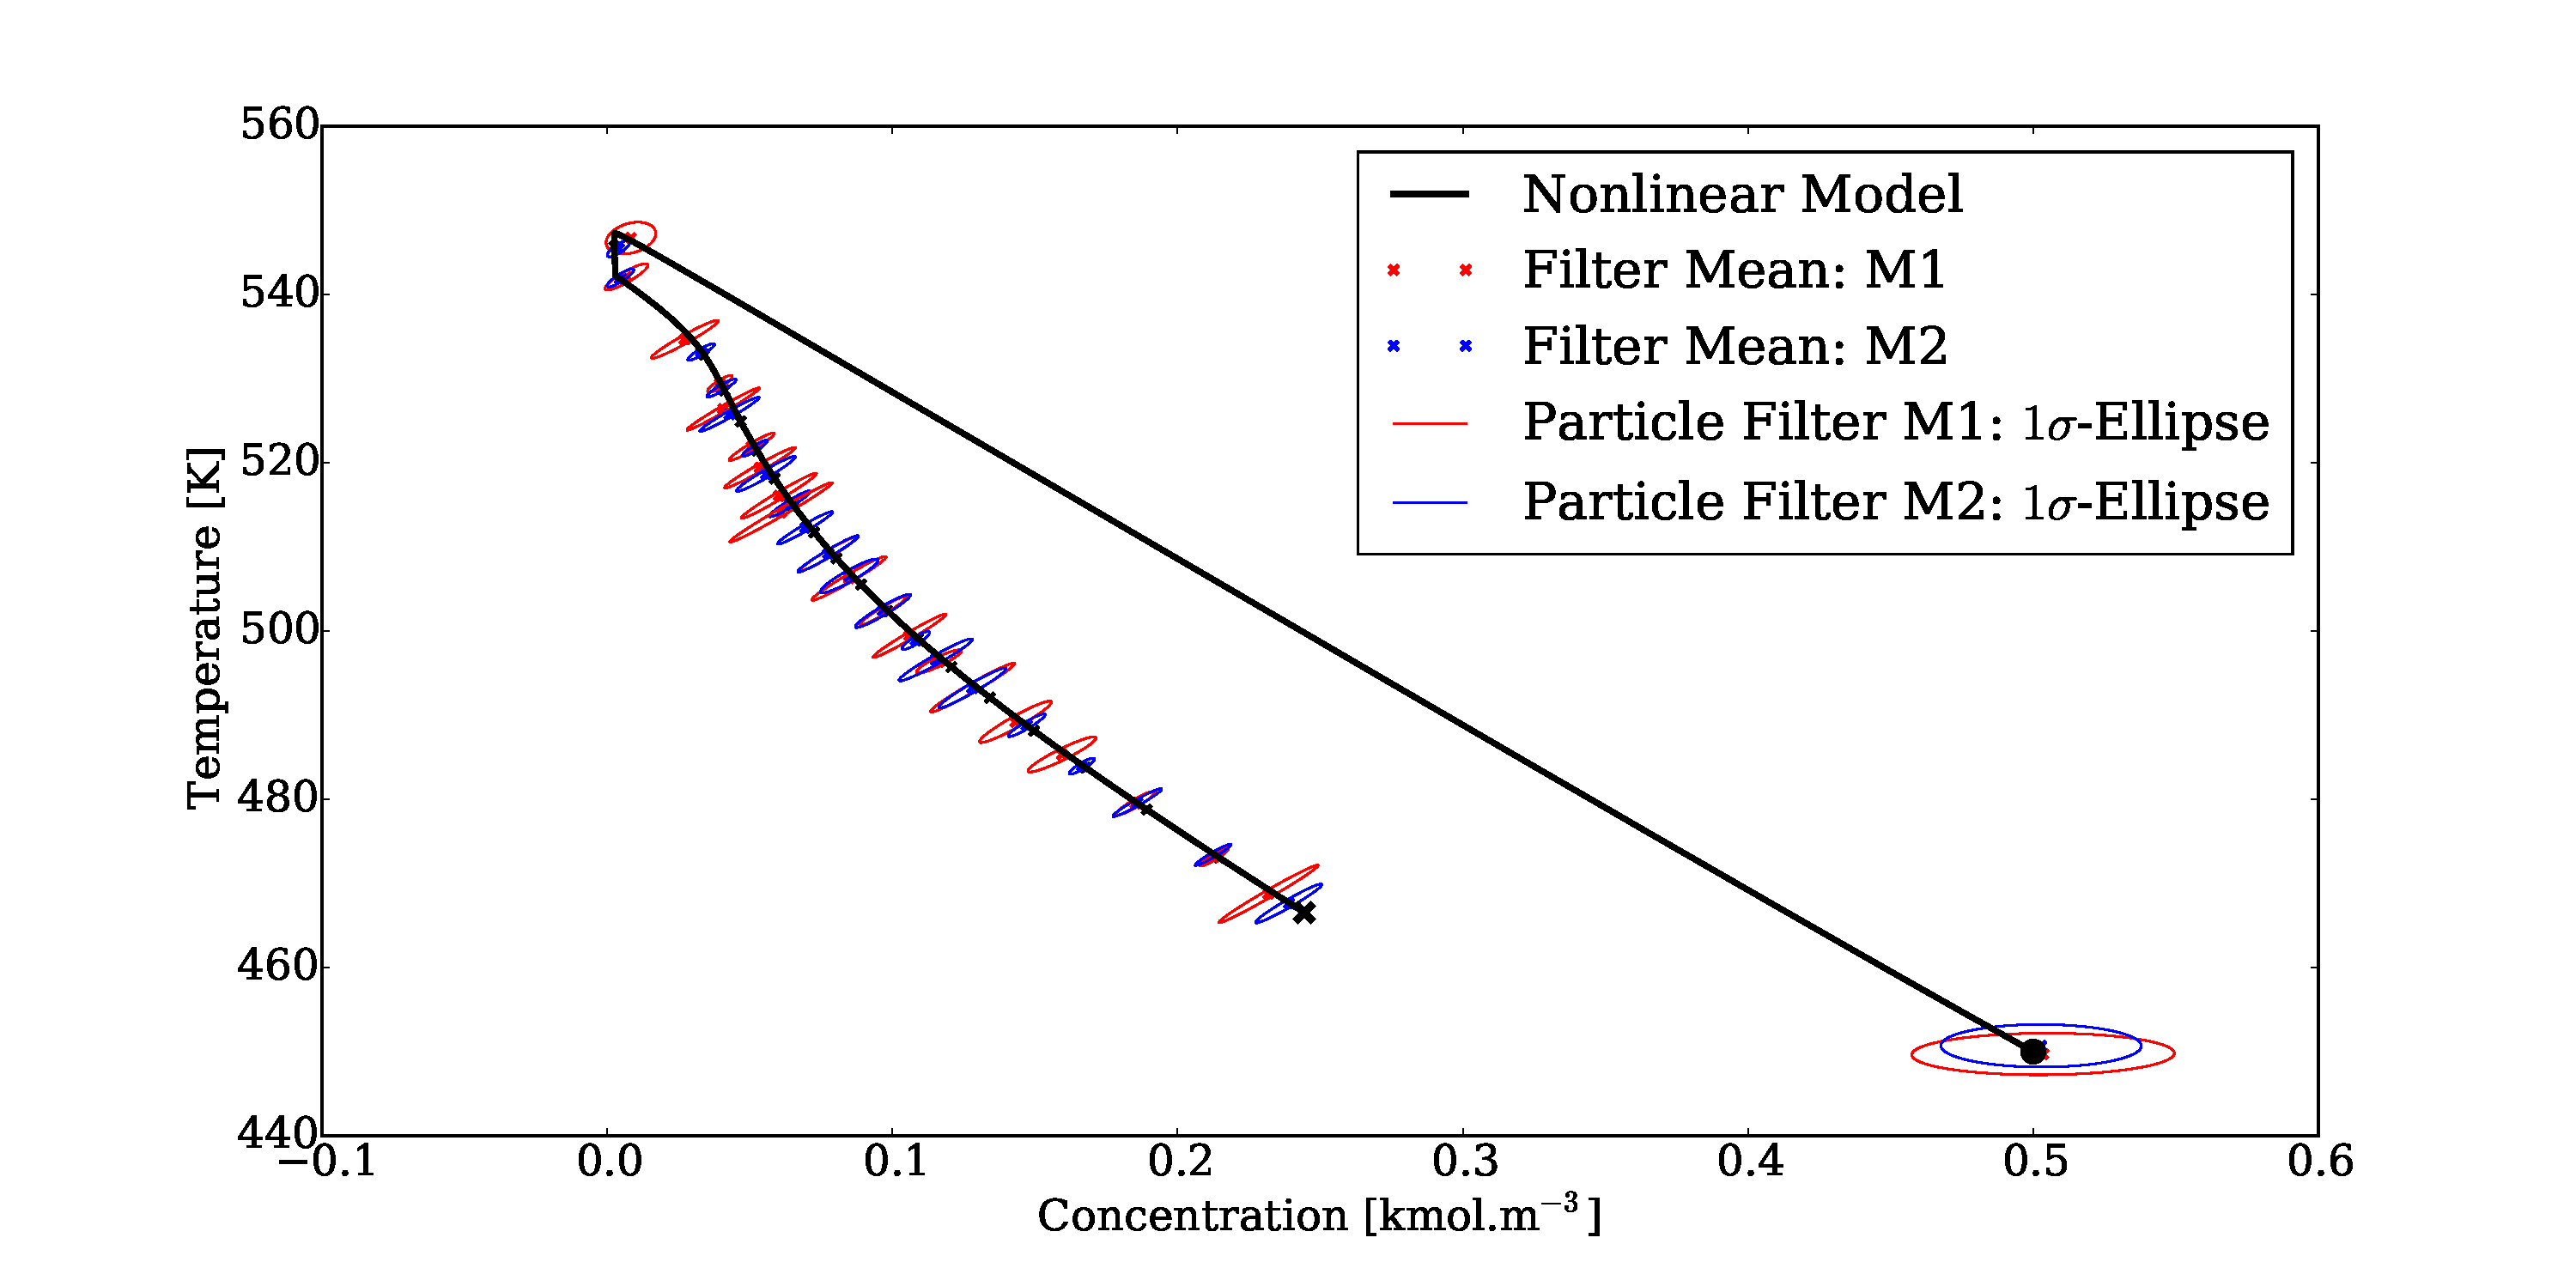
\includegraphics[scale=0.3]{spf_m1_m2.pdf}
\caption{State space trajectory of the states with posterior state estimates and confidence regions superimposed thereupon. The blue curves correspond to a two measurement filter and the red curves to a single measurement filter.}
\label{fig_spf_m1_m2}
\end{figure}
Based on Figure \ref{fig_spf_m1_m2} it is clear that the second measurement does indeed increase the accuracy of the posterior state estimate. This is not unexpected because the second measurement allows the filter to weed out even more particles which do not support the observation i.e. are representative of the true underlying state.





\subsection{Controlling the CSTR}

\bibliographystyle{plain}
\bibliography{research}

\end{document}